\section{Side-by-side}
\label{sec:sbs}

As a viewer's reference note, the theoretical values are presented on the left and the simulation values on the right.

\begin{table}[h]
\begin{center}
  \begin{tabular}{|c|c|}
    \hline    
    {\bf Name} & {\bf Value [Hz]} \\ \hline
    $Z_{I1}$ & 640.4922\\ \hline
$Z_{O1}$ & 477.0475\\ \hline
$AV_{1}$ & 110.6998\\ \hline
$Z_{I2}$ & 15013.86\\ \hline
$Z_{O2}$ & 0.9327305\\ \hline
$AV_{2}$ & 0.9856738\\ \hline

    \hline
  \end{tabular}
  \begin{tabular}{|c||c|}
    \hline    
    {\bf Name} & {\bf Value [Hz]} \\ \hline
    uco & 3.106930e+06\\ \hline
lco & 7.923603e+00\\ \hline
bandwith & 3.106922e+06\\ \hline

    \hline
  \end{tabular}
  \caption{Comparison 1}
  \label{tab:comparison 1}
\end{center}
\end{table}
\FloatBarrier

As seen, all values are of the same magnitude, so the differences are minimal.

\begin{table}[h]
\begin{center}
  \begin{tabular}{|c|c|}
    \hline    
    {\bf Name} & {\bf Value [dB]} \\ \hline
    $Z_{I}$ & 640.4922\\ \hline
$Z_{O}$ & 2.9364\\ \hline
$AV$ & 107.21838\\ \hline

    \hline
  \end{tabular}
  \begin{tabular}{|c||c|}
    \hline    
    {\bf Name} & {\bf Value [dB]} \\ \hline
    z_in1 & 5.638527e+02,-8.44302e+01\\ \hline
gain & -7.85216e+01,-1.54185e+00\\ \hline
lco & 8.880418e+03\\ \hline
uco & 1.603742e+06\\ \hline
bandwith & 1.594862e+06\\ \hline
cost & 1.013002e+05\\ \hline
merit & -1.39209e-01,-2.73352e-03\\ \hline

    \hline
  \end{tabular}
  \caption{Comparison 2}
  \label{tab:comparison 2}
\end{center}
\end{table}
\FloatBarrier

The gains and impedances are also identical as observed in the table above.

\begin{figure}[h] \centering
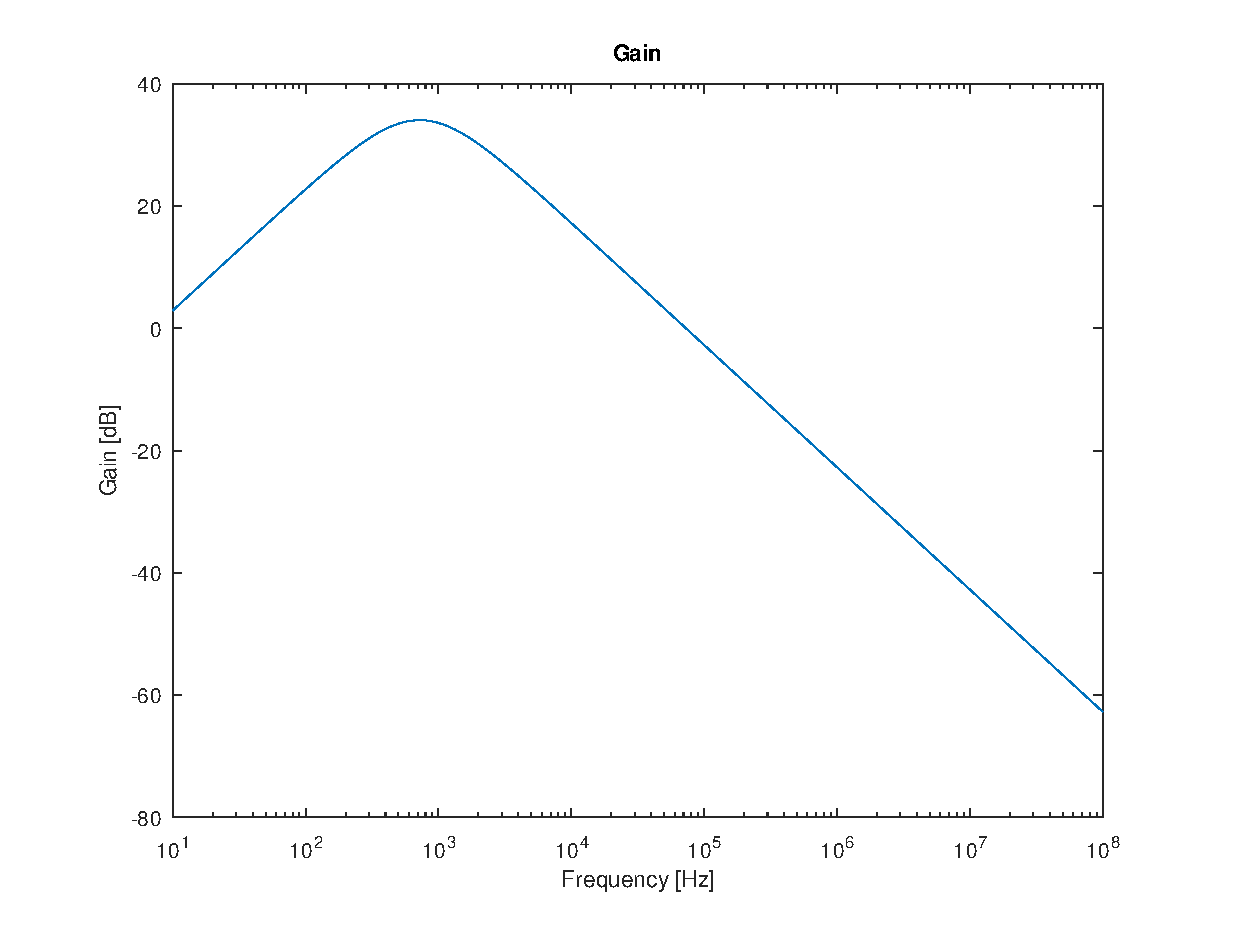
\includegraphics[scale=0.35]{teo_gain.eps}
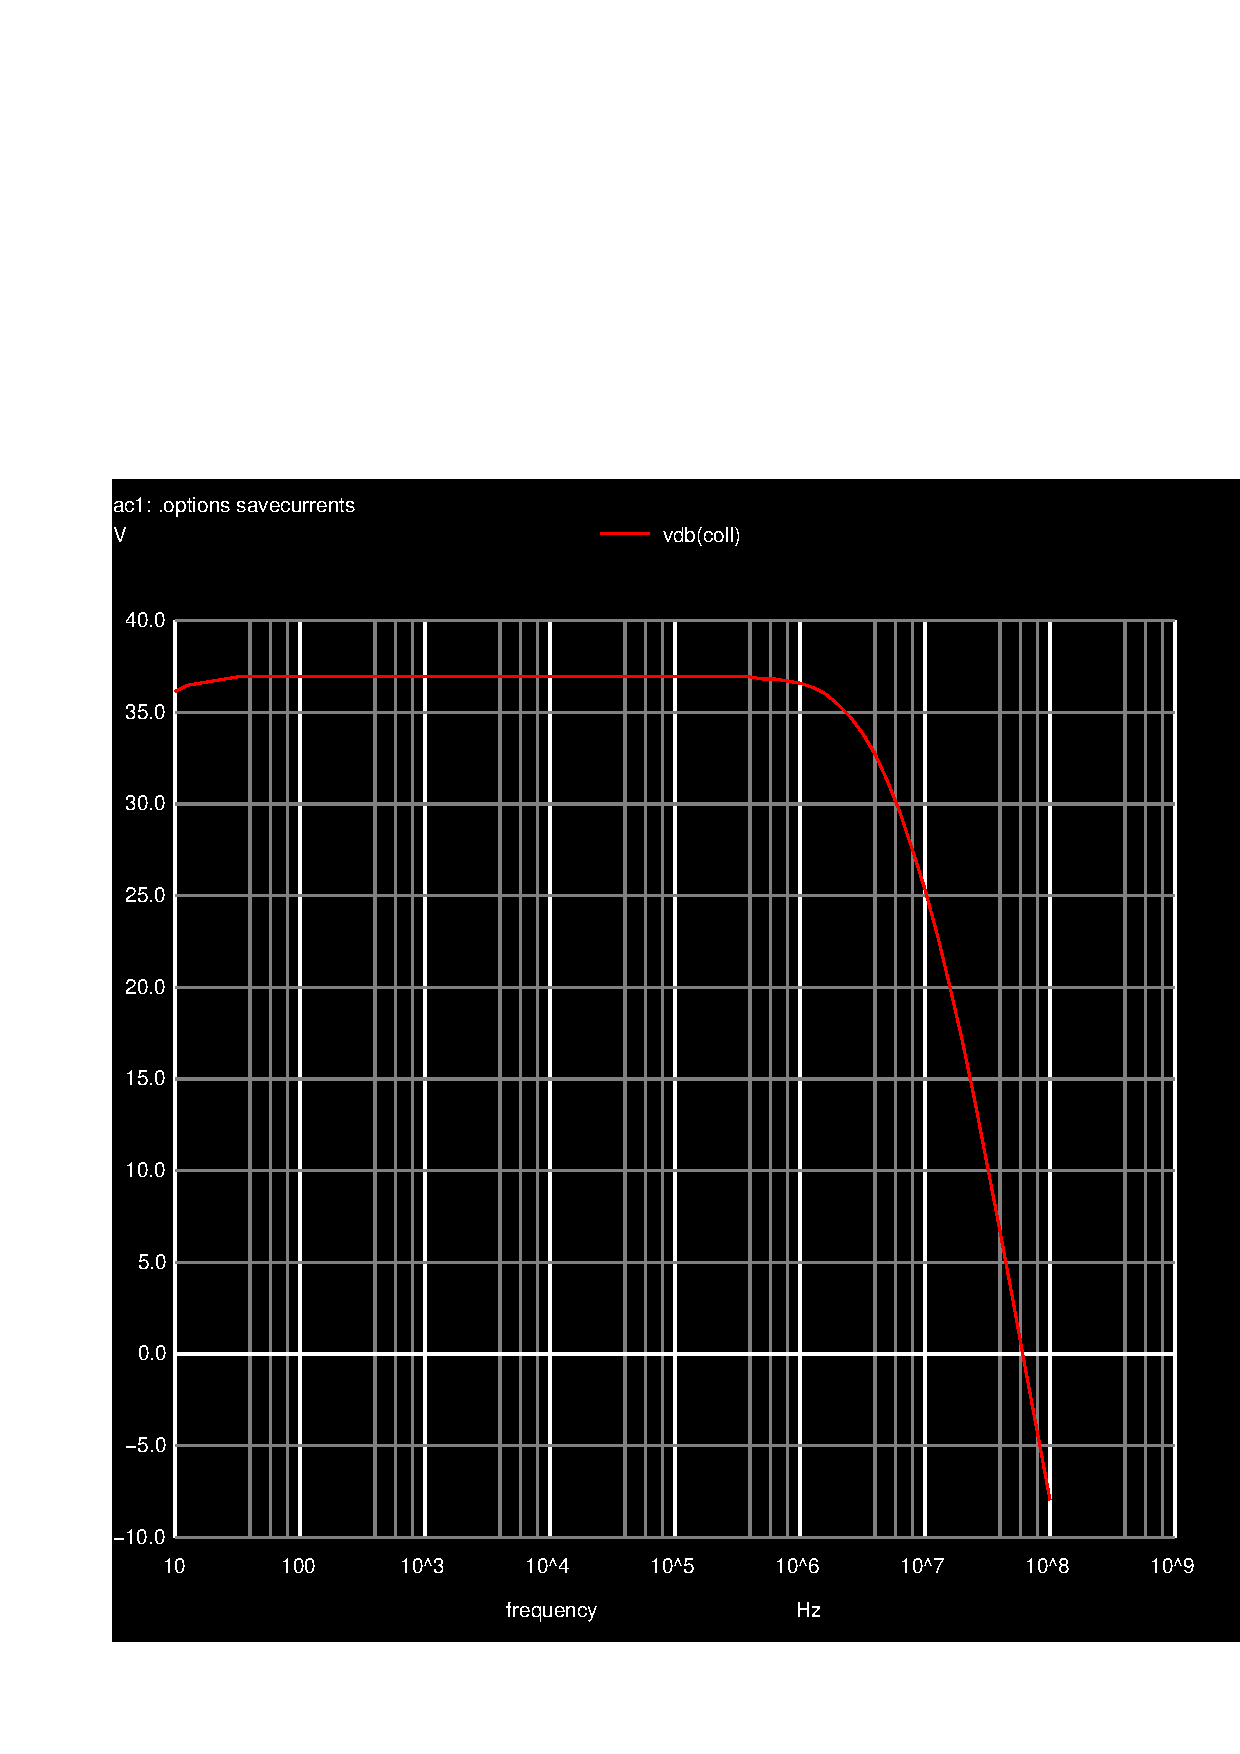
\includegraphics[scale=0.27]{vo1f.pdf}
\caption{Output voltage gain in order to frequency}
\label{fig:comparison 3}
\end{figure}
\FloatBarrier

The theoretical and simulated output voltage gain functions also behave identically, as observed in the plots.

\begin{figure}[h] \centering
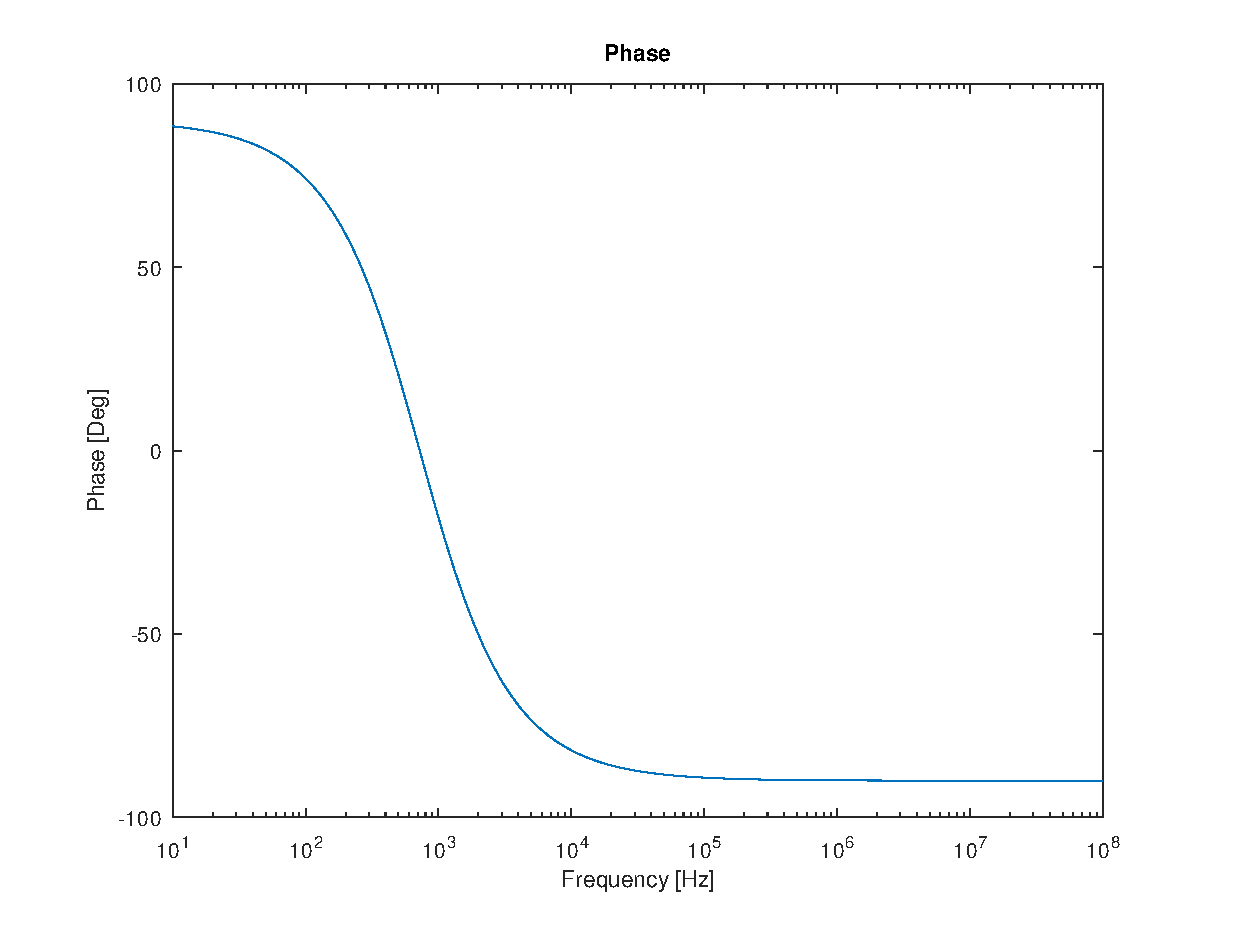
\includegraphics[scale=0.35]{teo_phase.eps}
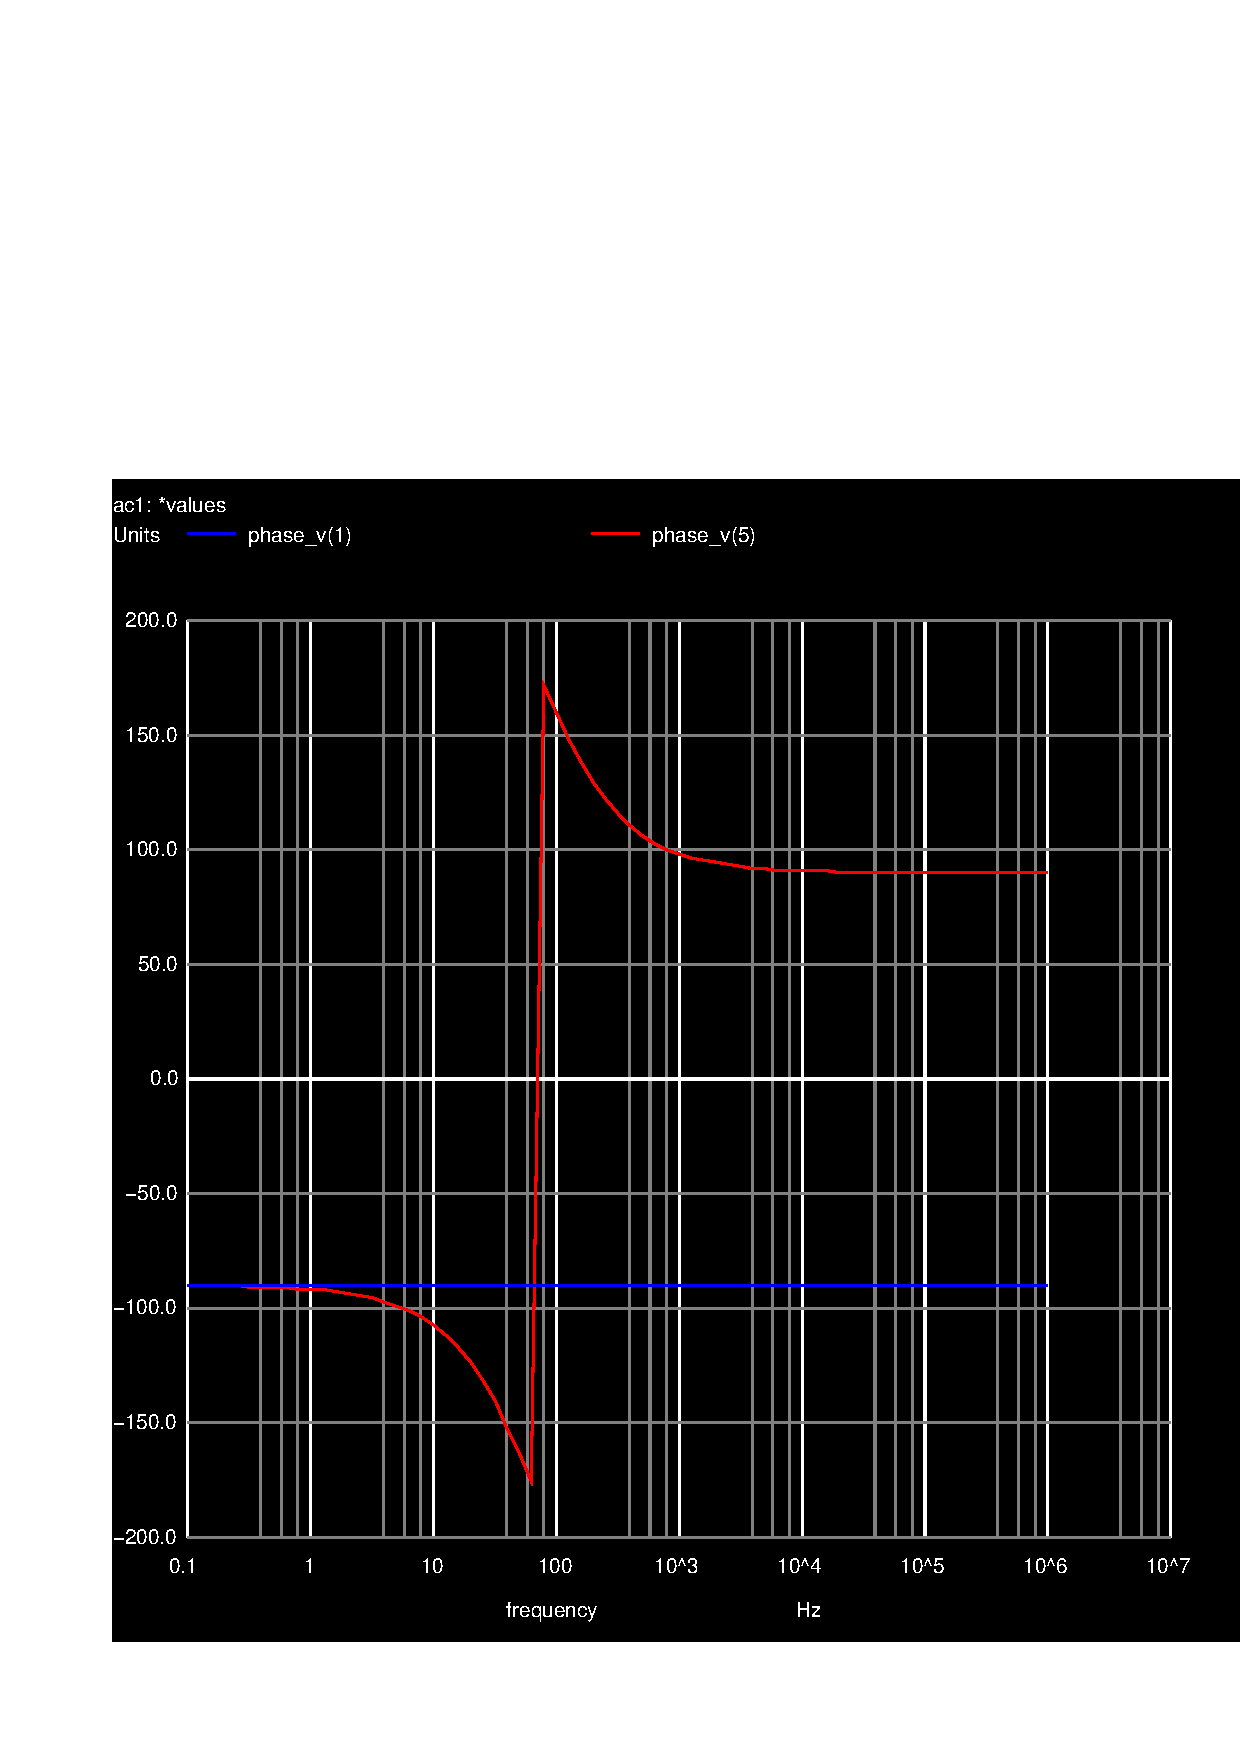
\includegraphics[scale=0.27]{phase.pdf}
\caption{Phase in order to frequency}
\label{fig:comparison 4}
\end{figure}
\FloatBarrier

The phase plots in order to frequency may seem different at first, but they show the same behavior: the amplitudes are 180 degrees on both plots, but the origin of the plots are in different spots.

\begin{table}[h]
\begin{center}
  \begin{tabular}{|c|c|}
    \hline    
    {\bf Name} & {\bf Value [Hz][Mu]} \\ \hline
    \input{../mat/data3_teo}
    \hline
  \end{tabular}
  \begin{tabular}{|c||c|}
    \hline    
    {\bf Name} & {\bf Value [Hz][Mu]} \\ \hline
    cost & 8.116008e+03\\ \hline
merit & 2.707518e+03\\ \hline

    \hline
  \end{tabular}
  \caption{Comparison 4}
  \label{tab:comparison 4}
\end{center}
\end{table}
\FloatBarrier

Here, apart from the frequency deviation and merit, all values are of the same magnitude. The simulation's merit is higher because of the frequency deviation, which is null in Ngspice's results, whereas in Octave it isn't.

\section{Conclusion}
\label{sec:conclusion}

All in all, this laboratory assignment showed that the difference between the theoretical models and the simulation is minimal, never differing significantly as seen in Section \ref{sec:sbs}. \par

This lab assignment showed us how to design a BPF circuit, which are widely used in wireless transmitters and receivers, being a key component in many contemporary applications. Once again, the in-person lab class gave us a hint of how the pratical approach differs from programmed simulations. \par

We consider that the merit achieved is frankly good, which means our circuit would be a good solution in terms of quality-cost relation for a company. In the end of the day, that will be one of multiple challenges in an engineer's life.



